%% ----------------------------------------------------------------
%% AppendixA.tex Circuit Diagrams
%% ---------------------------------------------------------------- 
\chapter{Circuit Diagrams} \label{Chapter:AppendixA:CircuitDiagrams}
\section{OV7670 Breakout Board Schematic}
\begin{figure}[ht!]
\centering
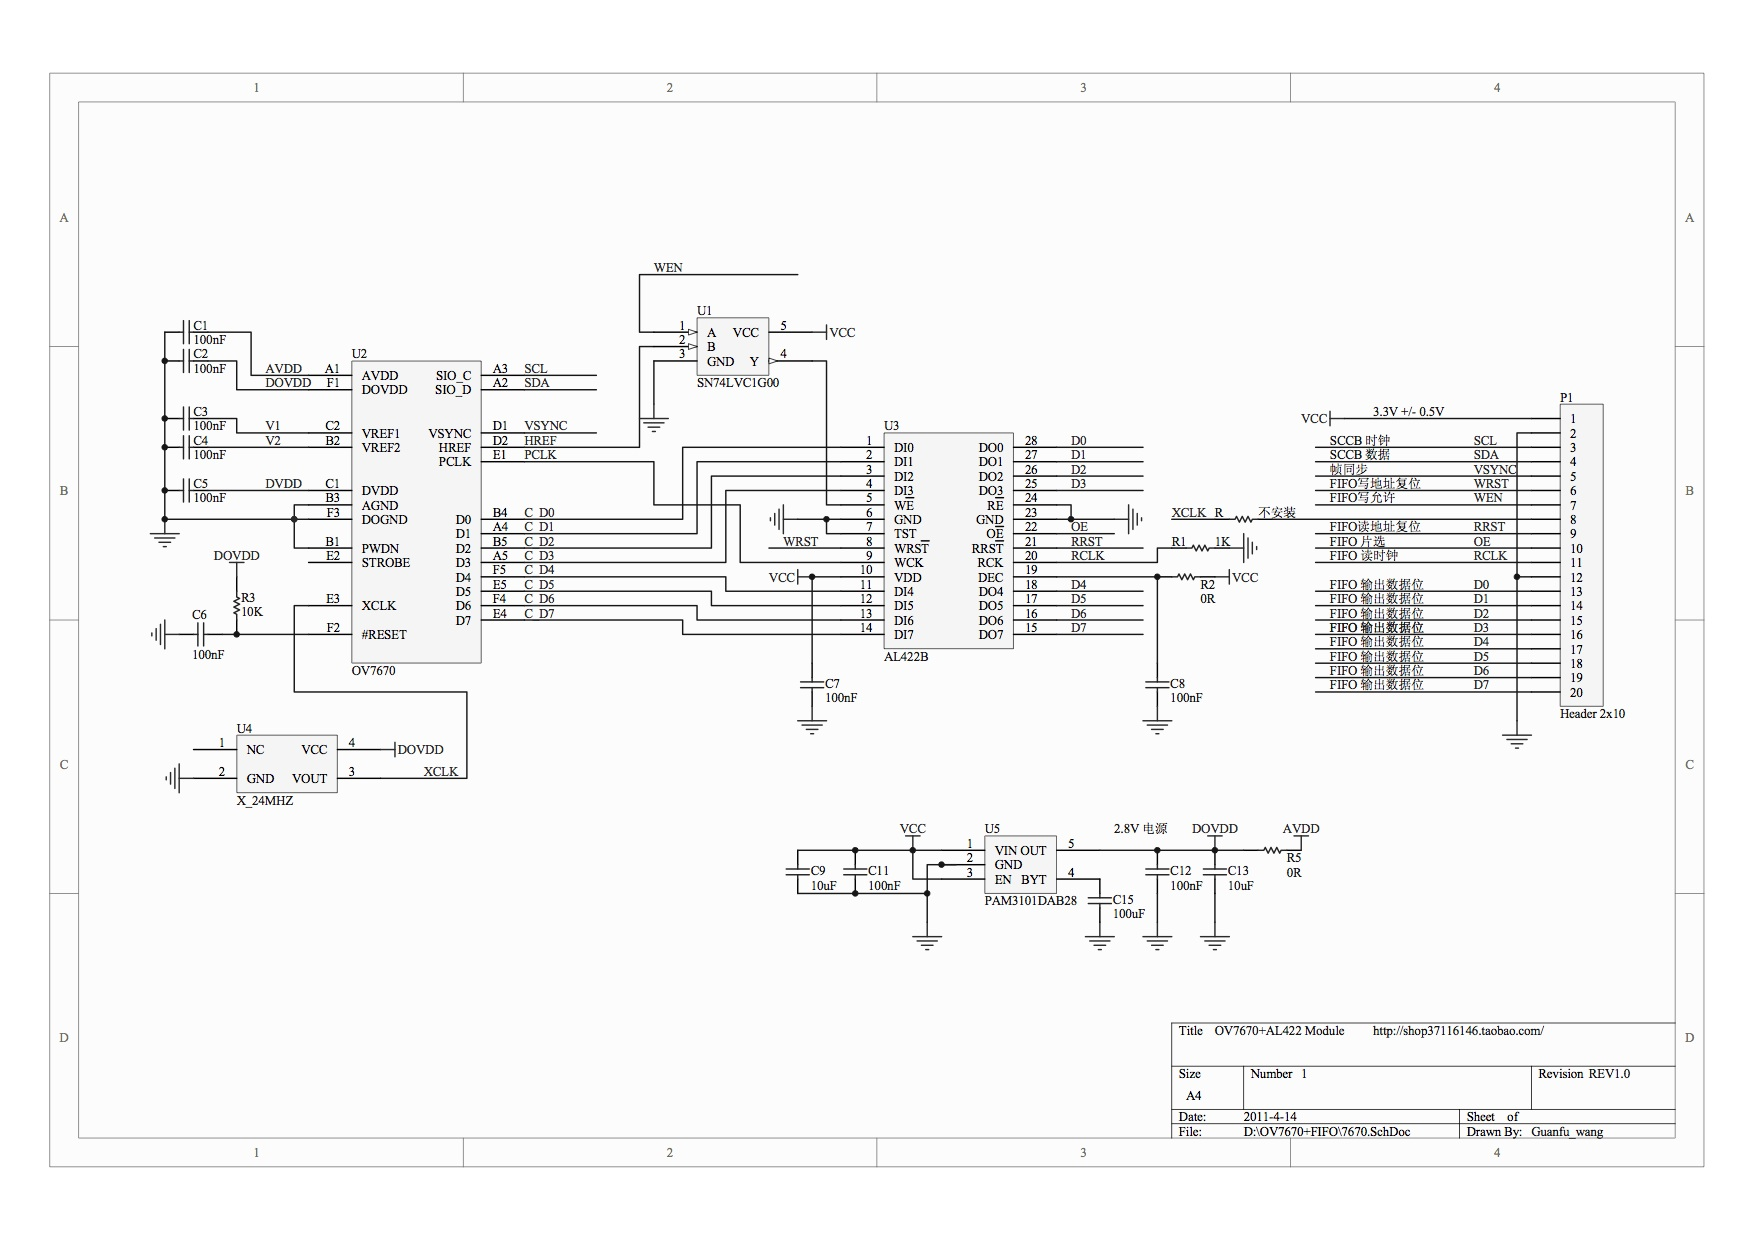
\includegraphics[angle=90,width=\textwidth,height=\textheight-10cm,keepaspectratio]{Figures/OV7670_Schematic.jpg} 
\caption{The circuit diagram for the OV7670 breakout board}
\label{OV7670_Schematic}

\end{figure}

\section{Il Matto and Dual Camera Schematic}
\begin{figure}[ht!]
\centering
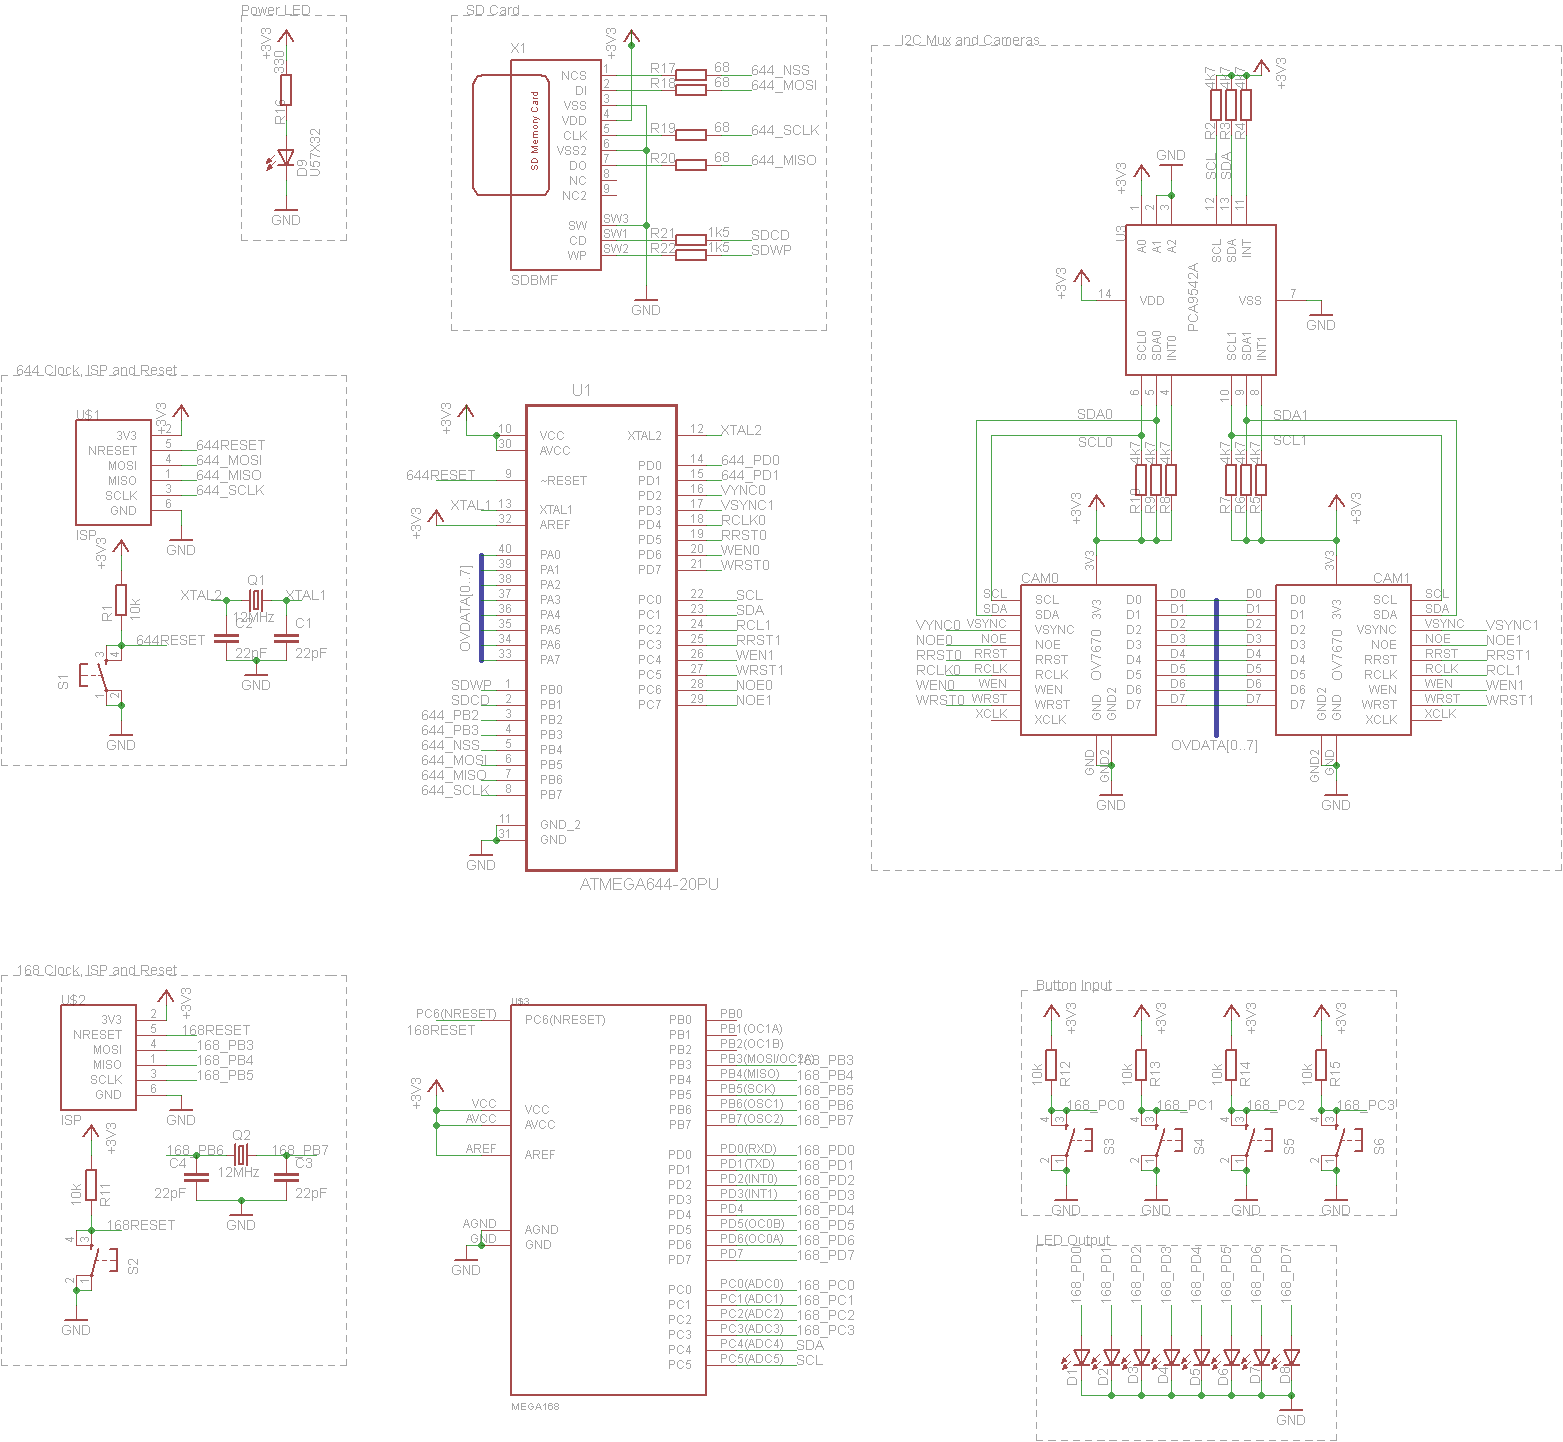
\includegraphics[angle = 90, width=\textwidth,height=\textheight,keepaspectratio]{Figures/IlMattoCamera_CircuitDiagram.png} 
\caption{The circuit diagram for Dual Cameras using the Il Matto Board}
\label{sch:DualCam_Schematic}

\end{figure}

\section{The Columbus Circuit Diagram} \label{sch:Columbus:CircuitDiagram}
\begin{figure}[ht!]
\centering
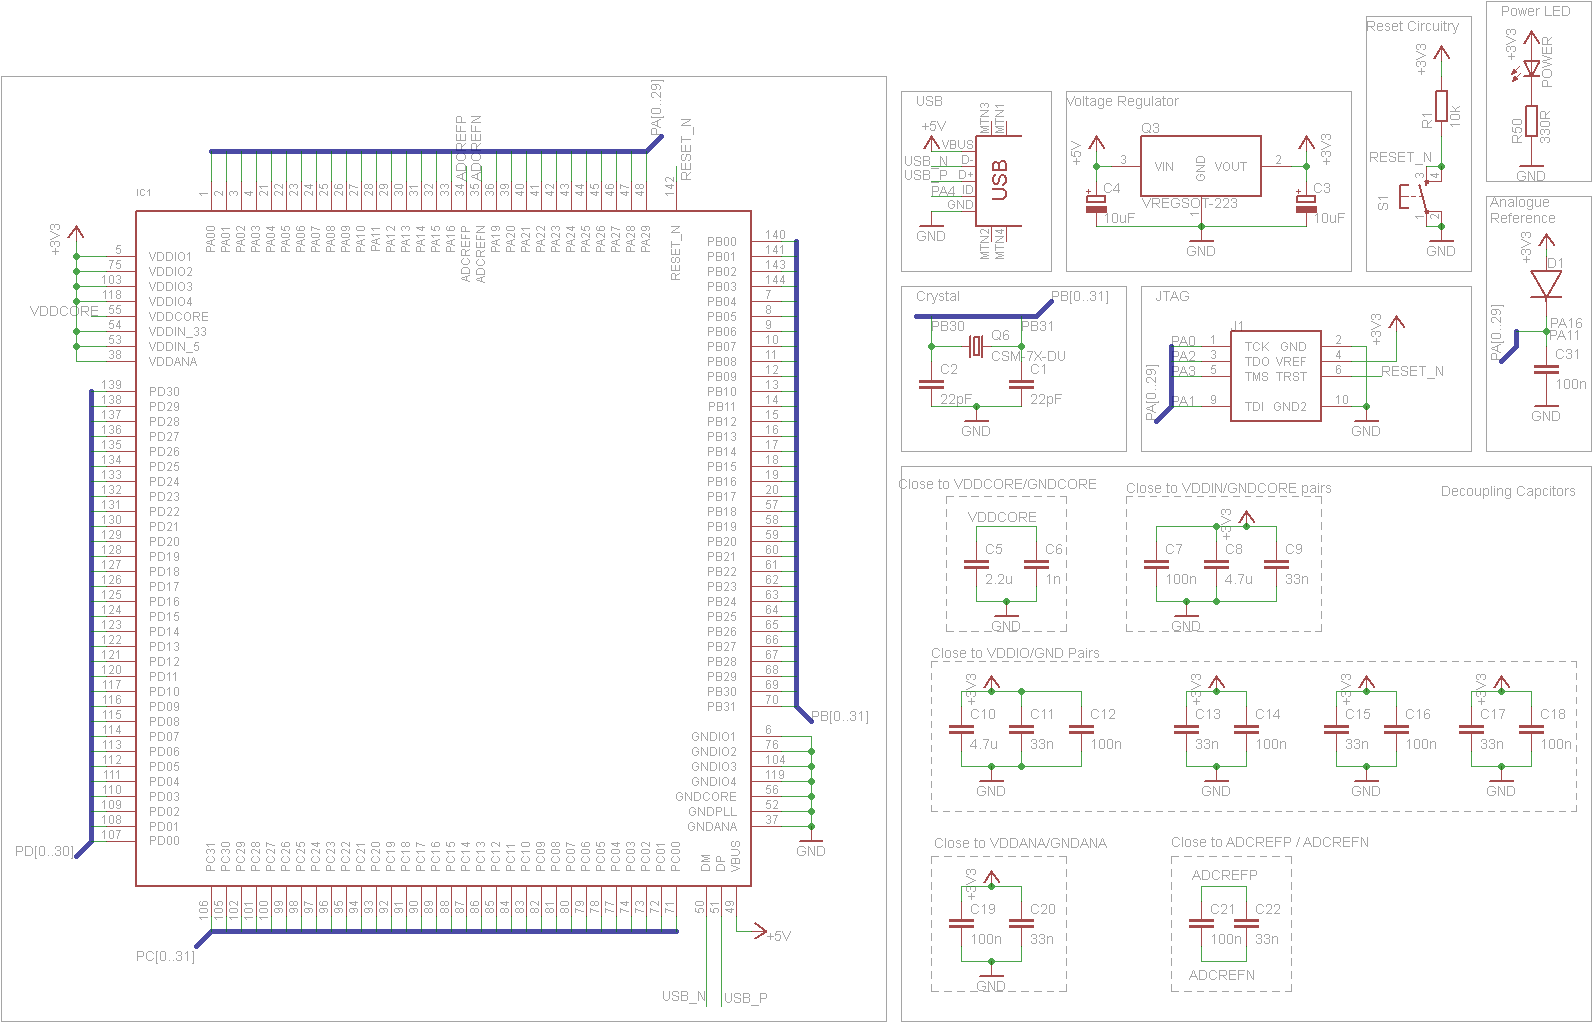
\includegraphics[angle = 90, width=\textwidth,height=\textheight,keepaspectratio]{./Figures/ColumbusCircuitPage1.png}
\caption{The Columbus Circuit Diagram Page 1}
\label{sch:Columbus_Schematic:1}
\end{figure}

\begin{figure}[ht!]
\centering
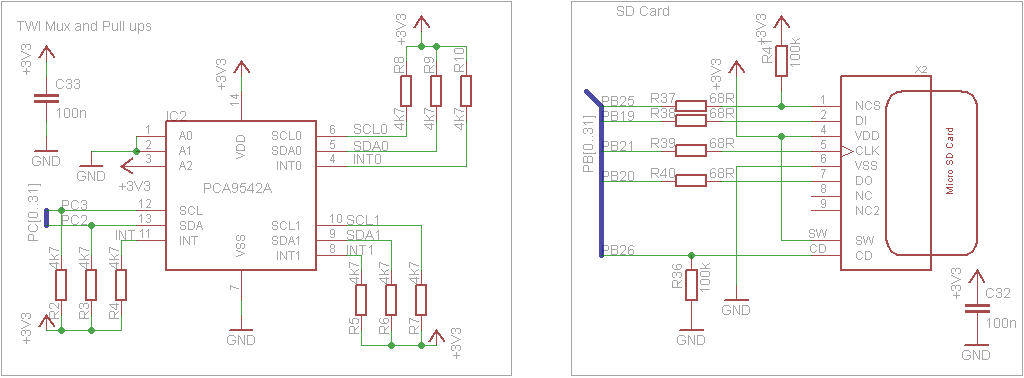
\includegraphics[angle = 90, width=\textwidth,height=\textheight,keepaspectratio]{./Figures/ColumbusCircuitPage2.png}
\caption{The Columbus Circuit Diagram Page 2}
\label{sch:Columbus_Schematic:2}
\end{figure}

\begin{figure}[ht!]
\centering
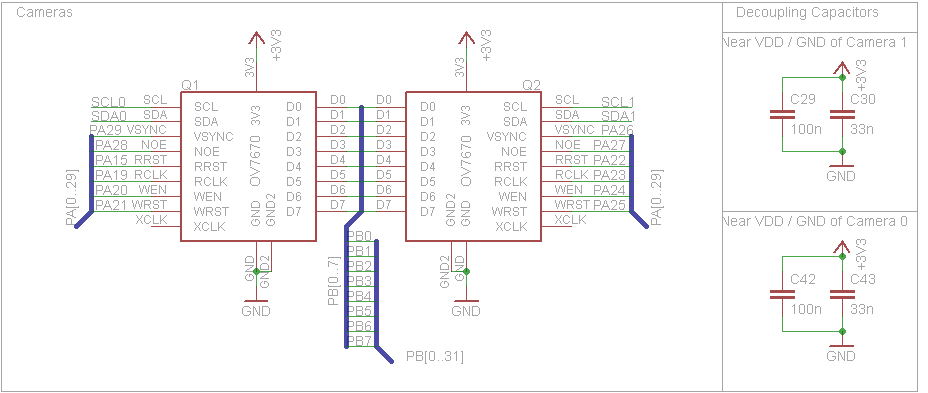
\includegraphics[angle = 90, width=\textwidth,height=\textheight,keepaspectratio]{./Figures/ColumbusCircuitPage3.png}
\caption{The Columbus Circuit Diagram Page 3}
\label{sch:Columbus_Schematic:3}
\end{figure}

\begin{figure}[ht!]
\centering
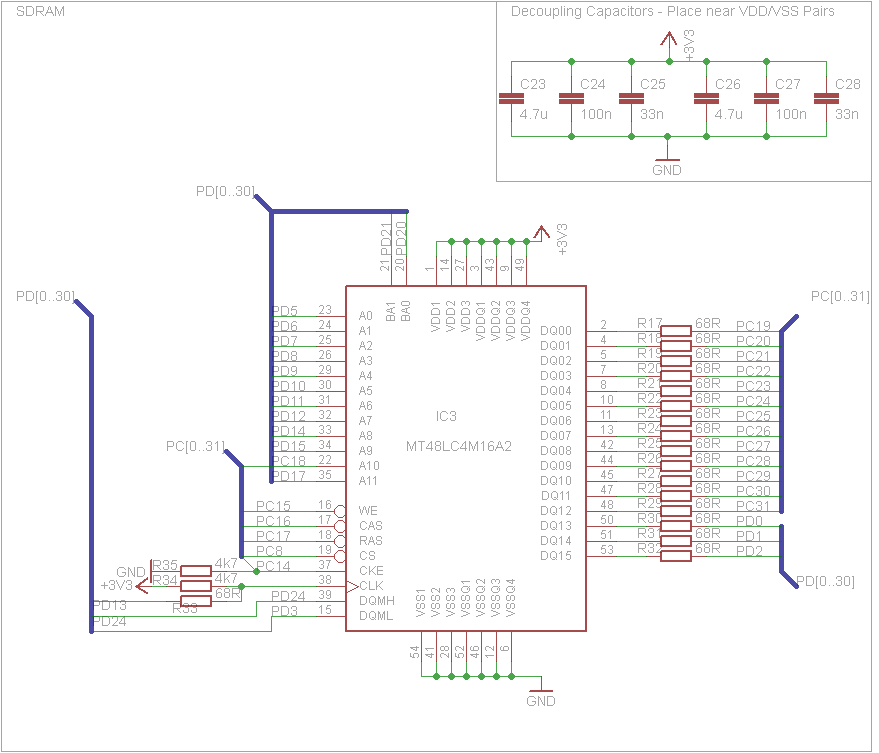
\includegraphics[angle = 90, width=\textwidth,height=\textheight,keepaspectratio]{./Figures/ColumbusCircuitPage4.png}
\caption{The Columbus Circuit Diagram Page 4}
\label{sch:Columbus_Schematic:4}
\end{figure}

\begin{figure}[ht!]
\centering
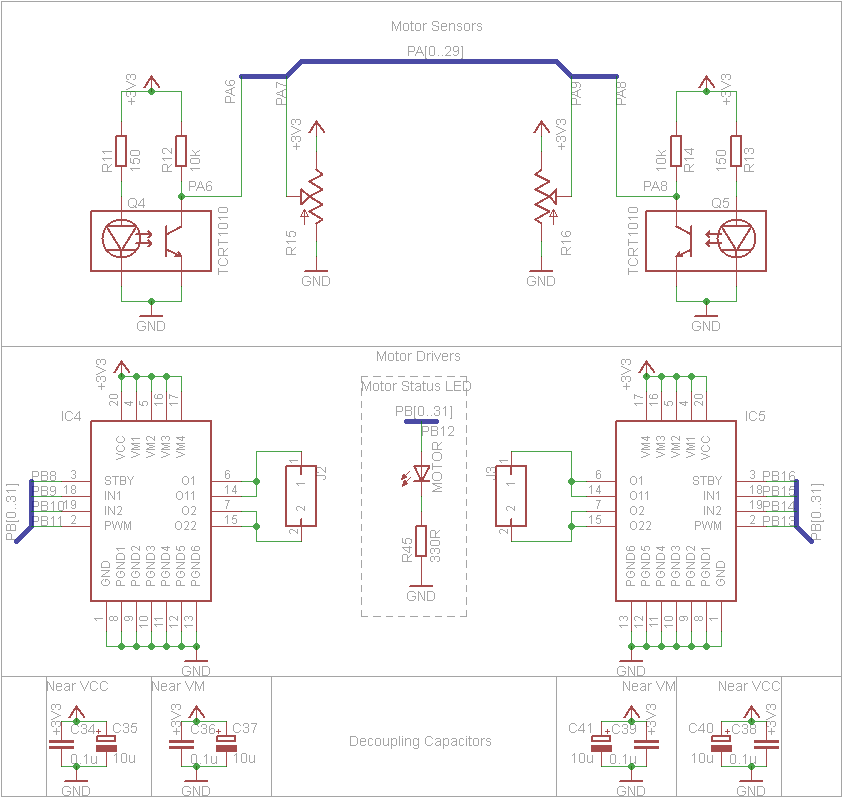
\includegraphics[angle = 90, width=\textwidth,height=\textheight,keepaspectratio]{./Figures/ColumbusCircuitPage5.png}
\caption{The Columbus Circuit Diagram Page 5}
\label{sch:Columbus_Schematic:5}
\end{figure}

\begin{figure}[ht!]
\centering
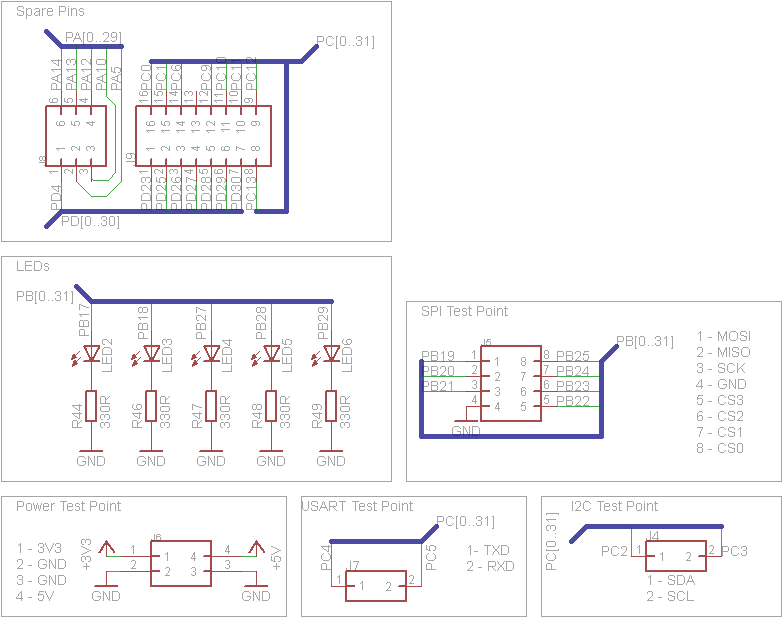
\includegraphics[angle = 90, width=\textwidth,height=\textheight,keepaspectratio]{./Figures/ColumbusCircuitPage6.png}
\caption{The Columbus Circuit Diagram Page 6}
\label{sch:Columbus_Schematic:6}
\end{figure}

